\chapter{Wymagania i narzędzia}
\label{ch:wymagania-i-narzedzia}

\section{Wymagania funkcjonalne}
Przy realizacji projektu powinny zostać spełnione następujące wymagania funkcjonalne:
\begin{itemize}
\item Poruszanie kamerą -
  użytkownik będzie posiadał możliwość zmiany położenia kamery oraz jej orientacji. Ponadto, będzie istnieć opcja kontrolowania kąta pola widzenia kamery.
\item Kontrola nad rozdzielczością obrazu -
  program pozwoli na konfigurację parametrów związanych z rozdzielczością renderowanego obrazu poprzez zmianę rozmiaru okna.
\item Użytkownik będzie miał wpływ na ustawienia parametrów związanych z~kształtowaniem terenu -
  w trakcie użytkowania programu dostępna będzie kontrola nad większością parametrów związanych z tworzeniem terenu.
\item Kontrolowanie parametrów związanych z renderowaniem terenu -
  projekt ten umożliwia dostosowanie ustawień mających wpływ
  na dokładność oraz jakość renderowania obrazu.
\item Interfejs graficzny -
  aplikacja wyposażona zostanie w graficzny interfejs użytkownika pozwalający na wykorzystanie dostępnej funkcjonalności programu.

\item Wyświetlenie średniego czasu renderowania sceny dla danych ustawień oraz ilość klatek na sekundę -
  interfejs aplikacji będzie na bieżąco przedstawiał informacje o~obliczonym średnim czasie renderowania pojedynczej klatki oraz ilości wyświetlanych klatek na sekundę.

\end{itemize}


\section{Wymagania niefunkcjonalne}
Wymagania niefunkcjonalne mają na celu zapewnienie:
\begin{itemize}
%% \item Odporności na niepoprawne dane wejściowe
\item Wsparcia dla wielu systemów operacyjnych - w tym Windows oraz Linux,
\item Wysokiej wydajności, poprzez wykorzystanie potoku programowalnego karty graficznej,
\item Weryfikacji ustawień podanych przez użytkownika.
\end{itemize}

\section{Przypadki użycia}
Diagram przypadków użycia został przedstawiony na rysunku \ref{fig:usecase}.
\begin{figure}[H]
\centering
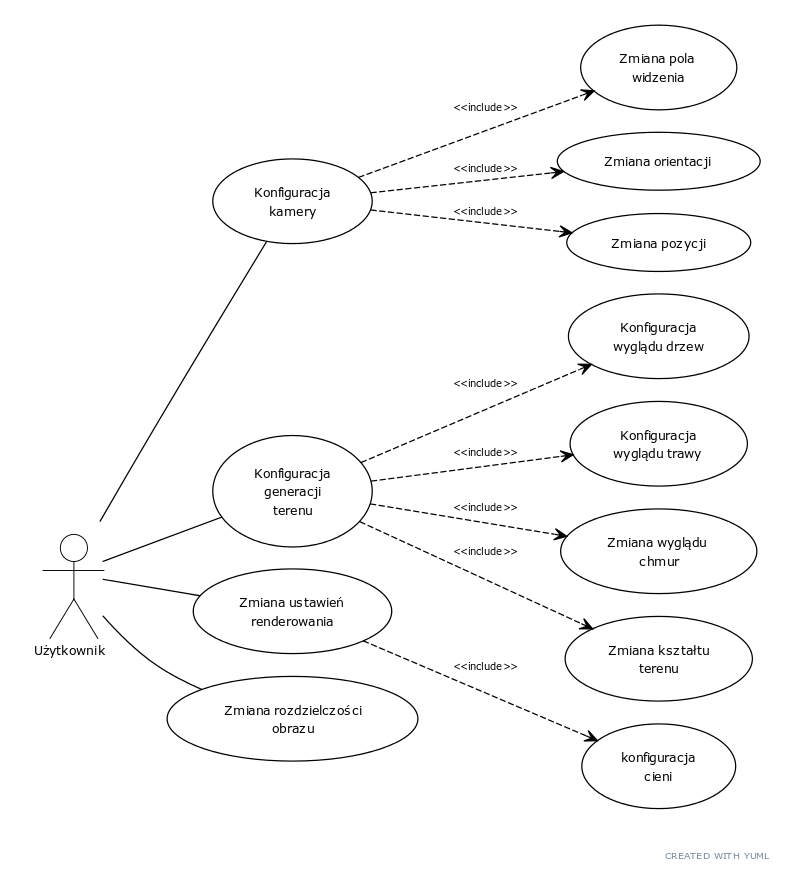
\includegraphics[width=1\textwidth]{./graf/usecase.png}
\caption{Diagram przypadków użycia.}
\label{fig:usecase}
\end{figure}

%% W programie nie znalazły zastosowania diagramy przypadków użycia.
\section{Wykorzystane narzędzia}

Do opracowania projektu wykorzystane zostaną narzędzia takie jak:
\begin{itemize}
\item gdb - Narzędzie  debugowanie programu,
\item valgrind - wykrywanie wycieków pamięci oraz profilowanie programu,
\item shadertoy.com - strona internetowa umożliwiająca tworzenie programów w~jednostce cieniującej fragmentów. Narzędzie zostało wykorzystane do~prototypowania i testowania różnych algorytmów i metod renderowania.
\end{itemize}

%% \begin{itemize}
%% \item opis narzędzi, metod eksperymentalnych, metod modelowania itp.
%% \item metodyka pracy nad projektowaniem i implementacją -- dla prac, w których ma to zastosowanie
%% \end{itemize}
